\documentclass[tikz,border=10pt]{standalone}
\begin{document}
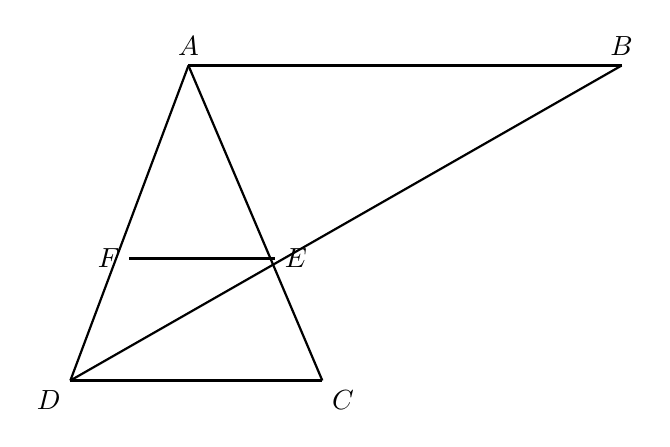
\begin{tikzpicture}[scale=1]
  \coordinate (A) at (1.5,4);
  \coordinate (B) at (7,4);
  \coordinate (D) at (0,0);
  \coordinate (C) at (3.2,0);
  \coordinate (F) at (0.75,1.55);
  \coordinate (E) at (2.6,1.55);

  \draw[thick] (A) -- (B);
  \draw[thick] (A) -- (D);
  \draw[thick] (A) -- (C);
  \draw[thick] (D) -- (C);
  \draw[thick] (D) -- (B);
  \draw[thick] (F) -- (E);

  \node[above] at (A) {$A$};
  \node[above] at (B) {$B$};
  \node[below left] at (D) {$D$};
  \node[below right] at (C) {$C$};
  \node[left] at (F) {$F$};
  \node[right] at (E) {$E$};
\end{tikzpicture}
\end{document}
